
\documentclass[11pt]{article}
 
\usepackage[margin=1in]{geometry} 
\usepackage{amsmath,amsthm,amssymb,xcolor,graphicx}
 
\newcommand{\N}{\mathbb{N}}
\newcommand{\Z}{\mathbb{Z}}
\usepackage{hyperref}
\usepackage{multirow}
 
\newenvironment{theorem}[2][Theorem]{\begin{trivlist}
\item[\hskip \labelsep {\bfseries #1}\hskip \labelsep {\bfseries #2.}]}{\end{trivlist}}
\newenvironment{lemma}[2][Lemma]{\begin{trivlist}
\item[\hskip \labelsep {\bfseries #1}\hskip \labelsep {\bfseries #2.}]}{\end{trivlist}}
\newenvironment{exercise}[2][Exercise]{\begin{trivlist}
\item[\hskip \labelsep {\bfseries #1}\hskip \labelsep {\bfseries #2.}]}{\end{trivlist}}
\newenvironment{problem}[2][Problem]{\begin{trivlist}
\item[\hskip \labelsep {\bfseries #1}\hskip \labelsep {\bfseries #2.}]}{\end{trivlist}}
\newenvironment{question}[2][Question]{\begin{trivlist}
\item[\hskip \labelsep {\bfseries #1}\hskip \labelsep {\bfseries #2.}]}{\end{trivlist}}
\newenvironment{corollary}[2][Corollary]{\begin{trivlist}
\item[\hskip \labelsep {\bfseries #1}\hskip \labelsep {\bfseries #2.}]}{\end{trivlist}}

\newcommand{\blue}[1]{\textcolor{blue}{#1}}

\newenvironment{solution}{\begin{proof}[Solution]}{\end{proof}}
 
\begin{document}

%%% I just yoinked this LaTeX template off Overleaf
 
\title{4803 Project Report: Evaluating N-Gram Models for Sentence Generation on Differently Sized Datasets}
\author{Ryan Rodriguez and Joseph Olaogun}

\maketitle

\section{Introduction}

With the recent research and public attention around large language models, machine learning and natural language processing are more important than ever to understand.  We aim to understand a core language model concept, N-Gram, as well as implement it mostly from scratch and evaluate its effectiveness in completing sentences when trained on datasets of varying sizes. \\

Our project answers the following research questions: \textit{What is an N-Gram model?  How can we account for words outside the scope of its original text?  How do we evaluate its performance?  How do these models perform on sentence generation tasks when trained on differently sized datasets?}\\

Our project is a hybrid of project types 1 (theory) and 2 (application): while we cover topics not discussed in detail during class, we will also evaluate performance based off relevant real-world datasets. We used the text of "The Cat in the Hat" for our small dataset \cite{seuss1957cat}, and "A Tale of Two Cities" for our large dataset \cite{pananjady2024just}.\\

We selected "The Cat in the Hat" due to its limited vocabulary, small size, and frequent use of rhyme.  Evaluating our model on a text with rhyme allows us to more easily determine whether a generated sentence is "accurate"
or not: "The Cat in the House" does not rhyme, and would be less desirable than a prediction like "The Cat in the Hat" (which rhymes). \\

We selected "A Tale of Two Cities" primarily due to its size.  It contains 135,409 words (as compared to "The Cat in the Hat", which has 1,624), which offers a significant advantage in training.  However, the text's sentence complexity and word variety may make prediction more difficult.

\section{N-Gram}
\label{sec:eval}

An N-Gram model is a simple language model that uses prior probabilities to predict which words come next from a starting window of words.  It runs a sliding window of length n through the training text, and records the frequencies of each word combination that follow.  Then, it randomly selects a word from the weighted frequencies of word choices seen in the training text (as depicted in Equation \ref{eq:noksmooth}), and continues until it reaches a set length of words.

\begin{equation}
\label{eq:noksmooth}
P(gram) = \frac{count(gram) }{total~count}
\end{equation} \vspace{0.1em}

As an example in this section, let's use the quote \textit{"There are things we know, things we think we know, and things we only know we do not know"} from Donald Rumsfeld as the training text for a model.  This is a very small instance for building a practical model, but it helps to demonstrate the concept.\\

By selecting the value of n, we can control the context window.  Figure \ref{fig:smooth} shows context results for setting $n=1$ (left) and $n=3$ (right).  Each line has a given window of words (e.g. "we" in the $n=1$ column) and frequencies of the words that appear next in the training text ("know" appears twice, while "think", "only", and "do" appear once).  The \texttt{<s>} and \texttt{</s>} characters are start and stop characters respectively, so that a sentence can be generated from scratch (the starting sequence only contains \texttt{<s>}) if desired.

% Joseph, for the life of me I cannot figure out how to insert <s> into the text without using \texttt.  Let me know if you can think of anything!

\begin{figure}[ht!]
    \centering
    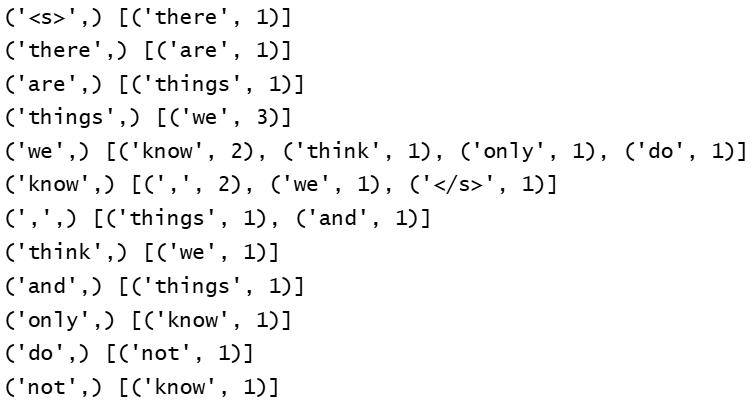
\includegraphics[width=0.49\textwidth]{smooth1.png}
    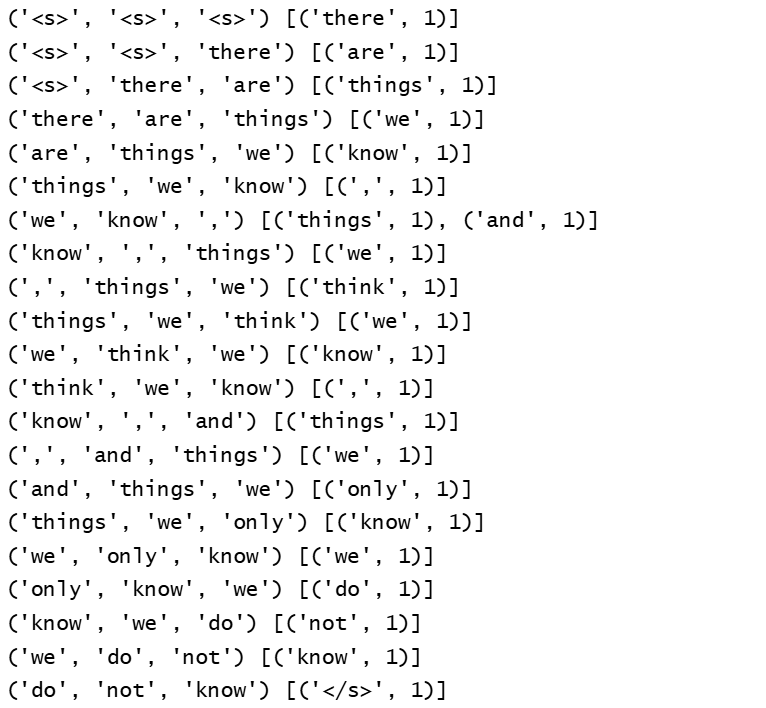
\includegraphics[width=0.49\textwidth]{smooth3.png}
    \caption{Contexts for $n=1$ (left) and $n=3$ (right).}
    \label{fig:smooth}
\end{figure}

Notice that as n becomes large, next word prediction becomes more and more deterministic, eventually just returning the original text verbatim. For example, running the models with an initial context of \texttt{<s> <s> <s>} (starting a new sentence) and a run length of 20 gives us:

\begin{figure}[ht!]
    \centering
    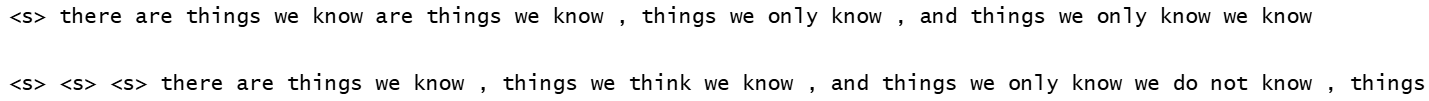
\includegraphics[width=1\textwidth]{two sentences.png}
    \caption{Contexts for $n=1$ (top) and $n=3$ (bottom).}
    \label{fig:contexts}
\end{figure}

As observed above, leaving the model as is presents several problems.  If the value of n is high, the training text is small, or the training text rarely repeats words, the model will tend to regurgitate sections of text exactly from the training text.  Additionally, the model is unable to deal with words outside of the training text vocabulary.  These two factors lead to poor generalization ability and a subpar model, as seen in Equation \ref{eq:noksmooth}.\\

To account for this, k-smoothing can be implemented to improve generalization, as seen in Equation \ref{eq:ksmooth}.  By setting $k > 0$, words that previously had no probability of being suggested now have a chance. Depending on your value of k, this can either help or hurt your model - large values of k increase the chance your model will spout gibberish, while very small values will function similarly to the model shown in Equation \ref{eq:noksmooth}.\\

\begin{equation}
\label{eq:ksmooth}
P_{k-smooth}(gram) = \frac{count(gram) + k}{total~count+k \cdot |vocab|}
\end{equation} \vspace{0.1em}

This approach still prevents words outside of the original vocabulary from being suggested, but that is a more complicated problem we chose to leave outside the scope of our project.\\

Model evaluation is another issue.  Identifying the "best" model is subjective, as it involves determining which sentences are more appropriate than others, and largely depends on the goals of the model.  We identified the following rough sub-goals to guide our evaluation metric search:

\begin{enumerate}
    \item Form semi-coherent sentences.
    \item Form phrases that sound similar to the author's voice.
\end{enumerate}

% Joseph, let's add more here as needed

One metric is \textbf{accuracy}, or dividing the total number of correct guesses over the total number of guesses made.  In our case, a sentence with low accuracy (e.g. "Green Eggs and Sam" rather than "Green Eggs and Ham") could still accomplish our goals of being coherent and retaining the author's original voice. \\

However, after discussions in office hours, we settled on using \textbf{parts of speech frequency} instead.  Making the tenuous (but somewhat supported by literature \cite{batanovic2015using}) assumption that two texts which have similar parts of speech frequencies are more similar, we developed a similarity score to gauge the similarity of generated text to its original training data.

\begin{equation}
\label{eq:sim}
similarity(g,t)= 1- \sum_{g_{pos}} |\frac{g_{pos}}{g}-\frac{t_{pos}}{t}| \cdot \frac{t_{pos}}{t}
\end{equation} \vspace{0.1em}

The similarity score shown in Equation \ref{eq:sim} aims to capture the weighted absolute differences between parts of speech frequencies.  By summing the differences in relative frequencies ($\frac{g_{pos}}{g} - \frac{t_{pos}}{t}$) for every part part of speech $g_{pos}$ in the generated text $g$, and then weighting it by the relative frequency of that part of speech in the training text ($\frac{t_{pos}}{t}$), this prevents outlier parts of speech from skewing the metric.  That total is subtracted from 1 to create a more familiar scale - if the two texts have identical distributions, they get a perfect similarity score of 1.\\

While this similarity score does not address whether sentences are coherent or not, we discovered that goal was very difficult to measure (both methods-wise and compute-wise) and settled on the similarity score as a proxy instead.  The similarity score primarily addresses the author's voice sub-goal.

\newpage
\section{Implementation}
\label{ref:implement}

One challenge of this project was implementing the methodology described above \textbf{almost entirely from scratch}.  We only used three python packages for our model and analysis: \texttt{random} (for random selection), \texttt{re} (for data pre-processing and cleaning), and \texttt{spacy} (which maps words to parts of speech from a pre-created dataset).\\

Our code for this project is available here: \blue{\href{https://github.com/rjacrod/4803proj}{https://github.com/rjacrod/4803proj}}\\

After testing, we discovered that unigram, bigram, and trigram models produced the most coherent predictions, likely due to the small size of our datasets. Because n-gram models rely on randomness to produce predictions, the quality of generated text and similarity score values varied between attempts.\\

To address this, we selected a generation length of 30 to allow generation of 1-2 sentences (we hypothesized a longer generation length reduces variability in part of speech frequencies) and ran 5 independent replications for each of the hyperparameter results we will display.  The similarity scores shown in the results are averaged over 5 iterations.\\

We also identified three k-smoothing values to use for our analysis: 0 (no smoothing), 0.5, and 1.  For the Cat in the Hat and Tale of Two Cities texts, this brings our possible hyperparameter values to:

$$n: \{1, 2, 3\} \hspace{0.5in} k: \{0, 0.5, 1\}$$

\section{Results}
\label{sec:results}

\subsection{The Cat in the Hat}

\begin{table}[!ht]
\centering
\begin{tabular}{lllll}
                            &                        & \multicolumn{3}{c}{\textit{k}} \\
                            &                        & 0          & 0.5          & 1         \\ \cline{3-5} 
\multirow{3}{*}{\textit{n}} & \multicolumn{1}{l|}{1} & 0.961          & 0.925            & 0.872         \\
                            & \multicolumn{1}{l|}{2} & 0.935          & 0.887            & 0.894         \\
                            & \multicolumn{1}{l|}{3} & 0.926          & 0.898            & 0.910        
\end{tabular}
\caption{Average similarity scores for \textit{The Cat in the Hat} hyperparameters}
\label{tab:cat}
\end{table}

The similarity scores for \textit{The Cat in the Hat} are in Table \ref{tab:cat}.  Models without smoothing ($k = 0$) had the highest similarity scores regardless of their $n$ value.  This makes sense, as \textit{The Cat in the Hat} is a very short text (roughly 1000 words), and a smoothness value of $k = 0.5$ or $k=1$ would drown out the context window by heavily weighting random chance.\\

Indeed, we can see this in the bigram model with $k=1$: as shown in Figure \ref{fig:gibberish}, the model returns gibberish with a relatively low similarity value (0.889).

\begin{figure}[ht!]
    \centering
    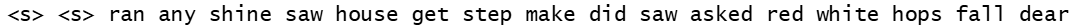
\includegraphics[width=1\textwidth]{gibberish.png}
    \caption{High values of k produce gibberish.}
    \label{fig:gibberish}
\end{figure}

Decreasing our k to $k=0$, unigram, bigram, and trigram models return somewhat more coherent phrases, as seen in Figure \ref{fig:trio}.  The unigram model shows the most promise here, with recognizable phrases like "these things net her the cat" and "i saw him".  It also observed the highest similarity score.  Shorter phrases are visible in the bigram model output, like "the wet red things", but are not as obvious as in the unigram model.

\begin{figure}[ht!]
    \centering
    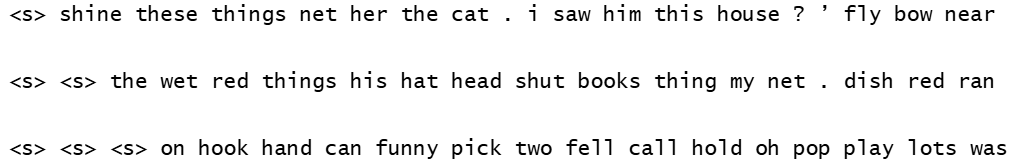
\includegraphics[width=1\textwidth]{trio.png}
    \caption{Low values of k and n produce more recognizable phrases.}
    \label{fig:trio}
\end{figure}

Finally, the trigram model has nearly no recognizable phrases (two word combinations like "two fell" or "oh pop" are likely due to random chance because of the training text's limited vocabulary) and performed similarly to the unigram model for $k=0.5$.  Looking at the context for the trigram model, only 137 trigrams have more than one choice out of 1536 total trigrams (8.9\%).

\subsection{A Tale of Two Cities}

\begin{table}[!ht]
\centering
\begin{tabular}{lllll}
                            &                        & \multicolumn{3}{c}{\textit{k}} \\
                            &                        & 0          & 0.5          & 1         \\ \cline{3-5} 
\multirow{3}{*}{\textit{n}} & \multicolumn{1}{l|}{1} & 0.902          & 0.876            & 0.889         \\
                            & \multicolumn{1}{l|}{2} & 0.878          & 0.880            & 0.873         \\
                            & \multicolumn{1}{l|}{3} & 0.888          & 0.875            & 0.883        
\end{tabular}
\caption{Average similarity scores for \textit{A Tale of Two Cities} hyperparameters}
\label{tab:tale}
\end{table}

A different trend emerged for\textit{ A Tale of Two Cities}, as seen in Table \ref{tab:tale}.  The lower overall similarity scores are to be expected, as it is a much larger dataset with more sentence complexity and parts of speech variety.  However, there is also lower variability between scores, with little difference between choices of $n$ for $k = 0.5$ and $k=1$.\\

The highest performing model was again the unigram model with $k=0$, which had recognizable phrases like "held her child", "had a certain", and "saw nothing was that as when":

\begin{figure}[ht!]
    \centering
    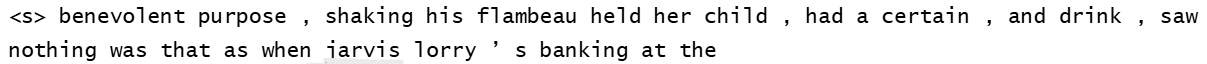
\includegraphics[width=1\textwidth]{goodmodel.png}
    \caption{Low values of k and n produce more recognizable phrases, as with\textit{ The Cat in the Hat}.}
    \label{fig:goodmodel}
\end{figure}

In this case, we believe the reason for poor bigram and trigram performance was the varied vocabulary used in \textit{ A Tale of Two Cities} - while bigram and trigram models can usually capture more complex trends, in this case there was insufficient training data to provide enough examples for the bigram and trigram models to train on.

\section{Conclusion}

This project explored the effectiveness of n-gram models with smoothing and parts of speech evaluation for use in sentence generation across different types of datasets.  We presented an evaluation metric for our models in Section \ref{sec:eval} and implemented an n-gram model mostly from scratch in Section \ref{ref:implement}. The results we present in Section \ref{sec:results} show that the effectiveness of n-gram models are very dependent on the characteristics of the initial datasets.\\

For the \textit{The Cat in the Hat} dataset, a unigram model with no smoothing was found to be most effective due to the limited size of the text.  Bigram and trigram models had insufficient training data, so for large values of $k$ the model usually resorted to random chance due to over-smoothing.\\

While the \textit{A Tale of Two Cities} dataset was very different from the \textit{The Cat in the Hat} dataset, a unigram model with no smoothing also performed the best.  Although the two cities text was much longer, more complex sentence structure and a highly varied vocabulary prevented the bigram and trigram models from producing meaningful predictions.\\

However, we showed that given sufficient useful training data, more complex n-gram models (large $n$) with non-zero smoothing should produce "better" sentences than unigram models with no smoothing.  Ideally, we would want a dataset that combines the best factors from each dataset: the limited vocabulary and simple sentence structure from \textit{The Cat in the Hat} combined with the length and varied sentences from \textit{A Tale of Two Cities}.\\

While simple models outperformed more complex ones in this case, we anticipate a larger, more suitable training dataset would produce different results.  Regardless, we feel this report presents a strong picture of understanding the theory of n-gram models, model implementation nearly from scratch, and evaluation of results in the context of the datasets and theory.

\newpage
\section{Statement of Labor}

Our project consisted of:
\begin{enumerate}
    \item A brief literature review of N-Gram models. (Ryan, Joseph)
    \item Identifying and pre-processing the differently sized datasets used for the project. (Ryan)
    \item Creating the N-Gram model, tuning n (full dataset length, bigram, trigram, etc). (Ryan, Joseph)
    \item Evaluating model performance and developing conclusions based off project results. (Ryan)
    \item Project writeup and report. (Ryan, Joseph)
\end{enumerate}

\bibliographystyle{plain}
\bibliography{references}

% \begin{figure}[ht!]
%     \centering
%     \includegraphics[width=0.5\textwidth]{1000_histogram_HW1.png}
% \end{figure}

\end{document}
